\documentclass{report}
\usepackage{graphicx}
\usepackage{listings}
\usepackage{amsmath}
\usepackage[pict2e]{struktex}
\usepackage{parcolumns}
\usepackage{pstricks}
\usepackage{enumerate}% to be able to customize enumeration lists 
% \usepackage{multicol}
%\usepackage[rflt]{floatflt}

%\usepackage{fullpage}

%I've found the following lines in the internet to automatically begin a new line after a paragraph
\makeatletter
\renewcommand\paragraph{\@startsection{paragraph}{4}{\z@}%
  {-3.25ex\@plus -1ex \@minus -.2ex}%
  {1.5ex \@plus .2ex}%
  {\normalfont\normalsize\bfseries}}
\makeatother

%to change section numbering depth to 3 (default 2)
\setcounter{secnumdepth}{3}

%to change depth for appearence in table of contents to 3 (default 2)
\setcounter{tocdepth}{3}

\begin{document}

% \documentclass[12pt]{article}

% \usepackage{ngerman}
% \selectlanguage{ngerman}
% \usepackage[latin1]{inputenc}

% \usepackage{graphicx}

% \begin{document}

\pagestyle{empty}

\begin{center}

\vspace*{-2.8cm}
\begin{minipage}[c]{.30\textwidth}
  \begin{flushleft}
    
\includegraphics[width=3cm,clip=]{LOGO/caltech_logo}%
  \end{flushleft}
\end{minipage}
\begin{minipage}[c]{.43\textwidth}
\vspace*{1em}
    {GALCIT (Caltech)\\Prof. Hans G. Hornung \\ \\ Institute of Aerodynamics (TUM) \\ Prof.~Dr.-Ing. N.~A.~Adams}%
\end{minipage}
\begin{minipage}[c]{.25\textwidth}
  \begin{flushright}
    \vspace*{1em}
    
\includegraphics[width=3cm,clip=]{LOGO/TUMLogo_oZ_Vollfl_blau_RGB}%
  \end{flushright}
\end{minipage}

\vspace*{3.3cm}
\begin{minipage}[c]{11cm}
{\LARGE\bf 
Simuation of high enthalpy flow in porosities using SPH}
\end{minipage}

\vspace*{0.8cm}
Oliver Oberinger\\

\vspace*{2.8cm}
{\bfseries Diplomarbeit}

\vspace*{1.2cm}
%\large
\normalsize
\vfill
\begin{tabular}{ll}
Betreuer: & ~Prof. Hans G. Hornung (Caltech)\\
\ & \ Dipl.-Ing. Sergey Litvinov (TUM)\\
 \\
Ausgabe: & 15.\ Juni 2010\\
Abgabe: & 15.\ Dezember 2010\\
\end{tabular}

\vspace*{1.6cm}
%\large
Institute of Aerodynamics Technische Universit\"{a}t M\"{u}nchen\\
Graduate Aerospace Laboratories California Institute of Technology\\
2010	
\end{center}

\pagebreak
\pagestyle{plain}

%\end{document}



\tableofcontents
\chapter{Introduction}
\label{sec:intro}


This work aims at the numerical simluation of high enthalpy flow over a porous
surface. The subject is of interest, as experients CITATION
NEEDED have shown that wall porosity can damp
acoustic instabilities in hypersonic flows over a slender cone. A numerical
simulation of this configuration is desired to furnish data for a detailed
analysis of the active mechanism. The simulation method of choice for the first approach
to this configuration is called Smoothed Particle Hydrodynamics (SPH). 

SPH designates a meshfree method for numerical simulation of particle
ensembles (respectively matter that can be modelled as an ensemble of
particles as is the case for fluids).
Thus, the term particle ensemble not only refers
to fluids (as the name of the method would suggest) but also to solids. In
fact nowadays SPH is employed to simulate problems in different fields,
such as elasticity and fracture of solids, liquid flows and gas
dynamics~\cite{Monaghan2005}.
The initial developement of the method dates back to 1977, when Gingold and
Monaghan tempted to compute an astrophysical gas dynamics problem with a new,
%%%%%%%%%%%%
% more MORE THAN WHAT

%correction:
%%%%%%%%%%%%%%%%
 compared to grid based methods more

efficient approach~\cite{Gingold1977}. Independently and simultaneously, work in
this field was also carried out by Lucy who came up with the same
idea~\cite{Lucy1977}.One main advantage of SPH, which also is the reason why SPH was applied first to astrophysical problems, lies in the fact that it is a particle method and therefore does not need any room-fixed grid for the underlying numerical scheme. Instead
the base for the calculation of derivatives are discrete points (particles), which move with the fluid (Lagrangian approach). Dealing with high density variations and huge calculation domains, astrophysical problems, when simulated with grid-based methods, 
required a considerable effort in terms of mesh-refinemend. For particle methods like SPH whereas, density variations are principally resolved naturally (more/less particles in a certain area) and calculation is only performed at places where there is matter (particles).
Another advantage is the relative ease of the
implementation of boundaries. And this is the main reason for the application of SPH in this work. For the structure of the solid boundaries represents a significant part of the problem, when treating porosities. 
 
%OTHER APPROACHES FOR CAVITY/POROSITY SIMULATION (look up in literature)
To be able to perform the simulation, a 2D compressible SPH code was developped in several stages and then tested for various test cases.
The first code that emerged from this project was a simple 1D compressible SPH code simulating a shock--tube problem. Although this code has no real use for practical applications, it is presented in this thesis with the goal to introduce the reader, who would like th familiarize himself with the implementation of SPH, to this technique.

The 2D code is based on an incompressible multi-phase SPH code, which was developed by HU and is now in use at the Institute of Aerodynamics of the TUM. This code was adapted in several steps to the needs of the present work, the first step being the implementation of the equations used in the 1D SPH code mentioned above and the adaption of the code to treat inviscid compressible problems. At this stage the code was tested for accuracy and robustness
by means of the 1D shock--tube problem. Both a 1D and a 2D particle distribution have been employed to this 1D problem. To conclude the 1D shock--tube tests, a study on the influence of perturbations in the particle distribution has been conducted, again both for 1D and 2D particle distributions.
At the same point, the simulation of acoustic wave propagation has been assessed, as acoustic phenomena are essential for the final flow configuration to investigate (see above).
Finally the code was further adapted to incorporate physical viscosity and heat conduction models.
...various test cases before simulating the actual porosity problem




\chapter{Method}
\label{sec:method}
\section{Basic Idea of SPH}
\label{sec:BasicsSPH}

To illustrate the basic idea of SPH, it is helpful to first consider the
governing equations of fluid dynamics, here represented by the Navier Stokes equations in
Lagrangian form (using the substantial derivative). The use of the Lagrangian form seems logical as SPH is a
particle method.

\begin {equation}
NAVIER STOKES IN LAGRANGIAN FORM
\end {equation}

The above equations have the form~\cite{Monaghan2005}

\begin {equation}
\label{eq:EFD_form}
{\frac{dA(r)}{dt}}=f(A(r),\nabla A(r),r)
\end {equation}
where
\begin {equation}
{\frac{d(.)}{dt}}={\frac{\partial(.)}{ \partial t}}+v\nabla(.)
\end{equation}
is the substantial derivative.

Thus the rate of change of  physical quantity depends on its spatial
derivatives. The goal of any method for numerical simulation is to approximate
these derivatives by information of a discrete number of points in order for a
computer to be able to handle it. 


The SPH method is based on the idea of approximating a function $A(x)$ by an
integral interpolant
\begin{equation}
\label{eq:int_interpolant}
A_I(x)=\int A(r')W(r-r',h)dr',
\end{equation}
where $W(r-r',h)$ is the so called kernel or smoothing function and $h$ the
smoothing length. If $W$ is the delta function this interpolation is exact,
otherwise it represents an approximation. As the theoretically
perfect kernel, the delta function, is of no practical use, the kernels
employed in practice are functions which tend to the delta function in the 
limit $h\rightarrow 0$.
Examples for those kernel functions are a Gaussian kernel or
kernels based on Schoenbergs~\cite{Schoenberg1946} $M_n$ splines~\cite{Monaghan2005}.
More detail on kernels is given in section
(LINK TO SECTION??) and in the book on SPH published by Liu~\cite{Liu2003}

The fact of using a kernel different from the delta function constitutes the
first of two approximations made by the SPH
method. It is often referred to as kernel approximation~\cite{Liu2003}.
The second approximation consists of a discretization of the integral
expression in equation~\ref{eq:int_interpolant}, thus changing the integraton
to a summation over all discretized elements (the particles) of the domain. 
This allows the determination of $A_I(x)$ by numerical methods. In the SPH
literature, this second approximation is commonly called particle
approximation~\cite{Liu2003}

With the relation between mass, density and volume for each discretized particle
\begin{equation}
m_i=\rho_i V_i,
\end{equation}
applying the particle approximation to \ref{eq:int_interpolant} leads to the following expression:

\begin{equation}
\label{eq:intInter}
A_S(r)=\sum_b m_b \frac{A_b}{\rho_b}W(r-r_b,h).
\end{equation}


In the same way, the derivative of the field function $frac{dA(x)}{dx}$ can be
approximated to give~\cite{Monaghan2005} or \cite{Liu2003} (in Liu with gradient,
im Monaghan for 1 direction)

\begin{equation}
\label{eq:simpleDerivative}
\nabla A_S(r)=\sum_b m_b \frac{A_b}{\rho_b}\nabla W(r-r_b,h).
\end{equation}

The disadvantage of the above equation \ref{eq:simpleDerivative} is, that for
$A(r)=const.$ the approximated derivative does not vanish. By writing (in
Monaghan the equation figures not with gradient but only in 1 direction!?!)
\begin{equation}
\label{eq:derivativeIdentity}
\nabla A = \frac{1}{\Phi}(\nabla {\Phi A}-A\nabla \Phi),
\end{equation}
where $\Phi$ is any differentiable function, this problem can be resolved. In its
SPH form  equation \ref{eq:derivativeIdentity} reads as follows:

\begin{equation}
\nabla_a A = \frac{1}{\Phi_a}\sum_b \frac{m_b}{\rho_b}(A_b-A_a)\nabla_a W_{ab}.
\end{equation}

It can be seen that the approximation to the derivative of the
field function $A$ is now expressed by a summation over the field function itself
and the derivative of the kernel function - which can be determined exactly.

Now the basic SPH formulations are introduced: Both the field function
itself and its spacial derivatives can be approximated using only information 
of a discrete number of particles. Hence, the rates of change of
the states described by the equations of fluid dynamics, which are of the form
\ref{eq:EFD_form}, can be rewritten using this information. Thus 
one obtains the SPH formulation of the equations of fluid dynamics.

The detailed derivation of the SPH equations for fluid dynamicy will not be shown here, as the
interest  only lies in describing the principle ideas behind the SPH
method. To summarize, these are as follows: A (field) function can be
described as an integral interpolation over the function itself and a kernel
function (which has to be chosen in an appropriate way). A further
approximation consists in transforming the integral over the domain into a
summation over the discrete elements (the particles) constituing this domain. 
This allows to express both
the field function and its spacial derivatives in forms 
that depend exclusively on discrete values
of the field function itself (and of the kernel function and its derivatives, 
all of which are known). By finally choosing an appropriate kernel function $W$ with
compact support (i.e. a finite support domain, where $W=0$ beyond) , the summation over all particles in the calculation domain can be reduced
to a summation over those particles within the support domain of the particle
in question.

The SPH formulation of the equations of fluid
dynamics is obtained by applying the above principles and conducting different
transformations to the original (exact) equations. Depending on the
transformations used, the final SPH equations can assume a different form. In
the following, a common form for the rates of change of density, velocity and
internal energy based on the EULER EQUATIONS (i.e. without viscosity and heat conduction)
is listed\cite{Monaghan2005,Liu2003} 
%(perhaps also list NSG-form, and
%explain why Euler is of interest as well (for 1DSPH code, perhaps later real
%code including viscosity???)

\begin{equation}
\label{eq:DCR_Euler}
\frac{d\rho _a}{\mathit{dt}}=\sum{m_{b}v_{\mathit{ab}}\nabla _{a}W_{\mathit{ab}}},
\end{equation}

\begin{equation}
\label{eq:VCR_Euler}
\frac{dv_{a}}{\mathit{dt}}=-\sum {m_{b}\left(\frac{P_{a}}{\rho_{a}^{2}}+\frac{P_{b}}{\rho _{b}^{2}}\right)\nabla_{a}W_{ab}},
\end{equation}


\begin{equation}
\label{eq:ECR_Euler}
\frac{de_{a}}{\mathit{dt}}=-\mathit{}\frac{1}{2}\sum{m_{b}\left(\frac{P_{a}}{\rho _{a}^{2}}+\frac{P_{b}}{\rho _{b}^{2}}\right)v_{\mathit{ab}}\nabla _{a}W_{\mathit{ab}}}.
\end{equation}

For the detailed derivation and for alternative formulations of
these equations refer to \cite{Monaghan2005, Liu2003}.



\section{Implementation of an SPH code}
This section presents some particular features of an SPH code. Emphasis is
placed on these features, that will finally be implemented in one of the
two SPH codes designed and modified during this work.
Points of interest are a closer description of the kernel function, different methods/algorithms to perform the search for the interacting particles, as well as the implementation of different boundary conditions in
SPH. Furthermore, different
equations of state are introduced, depending on the nature of the flow problem
to be considered (compressible/incompressible), followed by a passage
explaining the use of artificial viscosity. After this, some numerical
integration schemes that have proven to be reliable for SPH applications are discussed and the two different possibilities to calculate the density are shown. Finally a general structure of a generic SPH code is given




\subsection{Kernel function}
\label{sec:KernelFunction}
% ???not sure, if its the right place here, but somewhere there should be a
% paragraph with more detailed information on kernels used, compact support,
% perhaps even some properties,...(and perhaps some graphics???)


Some properties of kernel functions (smoothing functions) and notions related
to them have already been mentionned in section
\ref{sec:BasicsSPH}. In principle, every function can act as kernel function
if it respects a set of criteria listed by~\cite{Liu2003}.
The most important ones are:

The smoothing function should vanish outside of a certain area around its
center. This property is called compact support and the domain where $W\neq0$
is the support domain of the smoothing function. The smupport length $\kappa h$ and the
smoothing length $h$ are not to be confused.
 
\begin{equation}
W(x-x')=0,\textit{for}|x-x'|>\kappa h.
\end{equation}

The smoothing function should be normalized to 1, which ensures that constants
are interpolated exactly:
\begin{equation}
\int{W(x-x',h)dx'}=1.
\end{equation}

The smoothing function should tend towards the delta function as the smoothing
length $h$ tends to zero:
\begin{equation}
\lim\limits_{h \rightarrow 0}{W(x-x',h)}=\delta(x-x').
\end{equation}
This is to ensure consistency of the integral approximation, which means that
the approximate expression tends to the exact expression of the integral
interpolant equation for $h \rightarrow 0$.

The full list of SPH kernel properties can be found in  \cite{Liu2003}.
Based on those properties a variety of kernels are used in SPH literature. A
very commonly used kernel is the $M_4$ kernel (Cubic Spline) based on Schoenberg's
$M_n$-Splines~\cite{Schoenberg1946}.

\begin{equation}
\label{eq:cubicSpline}
M_{4}(x)=\begin{cases}
\frac{1}{6}[(2-q)^{3}-4(1-q)^{3}],& \text{for 0 $\leq$ q $\leq$ 1} \\
\frac{1}{6}(2-q)^{3},&  \text{for 1 $\leq$ q $\leq$ 2} \\
O,& \text{for q $>$ 2}.
\end{cases}
\end{equation}


In the work of \cite{Fulk1996} a measure of merit for kernels is developed and
they came to the result that, at least in 1D, no kernel performes significantly better
than the cubic spline.
This is why for the 1D SPH code described in section (\ref{sec:1DSPHcode}) the cubic
spline kernel was employed.

The unit of the kernel function $W$ is the inverse of the volume (or the corresponding 1D/2D magnitude), as can be seen easily from equation ~\ref{eq:SumDensity} which is only introduced below.


\subsection{Neighboring particle search methods}
\label{sec:NNPS}
To calculate the derivatives in \ref{eq:DCR_Euler}-\ref{eq:ECR_Euler} a
summation over all particles has to be performed. However, as we defined kernel
functions with a compact support, only particles within a certain distance from
the particle in question (within its support domain) contribute to the
interpolation of its values, and thus interact. Finding the interacting
particles is one of the key features in an SPH implementation, as an effective
interaction search method (often also called nearest neighboring particle (NNP)
search method in the SPH literature) can considerably reduce
computation time. 

The most basic NNP algorithm is called all pair search, and as its name
suggests all imaginable particle pairs are tested for interaction. This means
that the calculation process consists of a double loop where the outer loop
iterates over all particles and defines one of the pair's partners (often
refered to as origin). For each of the (origin) particles an inner loop is
performed, which iterates again over all particles thus defining the other
partner (destination) of the pair. Then, the pair is tested for the
interaction condition, meaning that their distance has to be smaller than the
support length. In this way, for a calculation domain consisting of $N$
particles, $N*N$ iteration steps and tests have to be executed. The
calculation cost of this approach is $O(N^2)$. 
If the
interactions are assumed to occur pairwise (i.e. if there is a spatially constant
smoothing (and therefore support) length; THINK ABOUT THE AVERAGED SMOOTHING
LENGTH...) there is a simple but efficient way of reducing computation
time. Thus, if a pair $P_{ij}$ is an interaction, the pair
$P_{ji}$ is an interaction as well. That way half of the $O(N^2)$ iterations
and tests can be eliminated, leading to a complexity of $O(N!)$ (LOOK FOR
REFERENCES). This approach is employed in the 1D SPH code as it is easy to
implement\cite{Liu2003} and the number of particles in this 1D simulation is
still reasonably low in order not to have to use more sophisticated algorithms
such as are introduced below.

A more effective but also more complicated method is the linked list
algorithm. This is based on the fact that kernels with compact support are
used and thus interacting particles may only be located in the neighborhood of
the particle under consideration. The computation domain is divided into cells (with
cell size$\ge \kappa h$, ideally $=\kappa h$), and the
particles are assigned to the cell they are located in~\cite{Monaghan1983}. In this way the cell
structure serves as a book--keeping device and in case of an interaction
calculation with an origin particle $i$ not all the particles $j,j={1,...,N}$ have
to be considered but only those particles in the adjoining cells. Hence, the
complexity of the original problem which is of order $O(N^2)$ can be reduced
considerably and even tends to $O(N)$ if the particles in one cell are few. 

FIGURE: DIAGRAM WITH CELLS /PARTICLES /DOMAIN!?!

Technically the cells are managed by the implementation of a linked list
structure in a computational code. More details on this are given in section
(SOMEWHERE IN 2D CODE DESCRIPTION), as this algorithm is implemented in the 2D
SPH code, and in \cite{Monaghan1985, Hockney1988}.
However, the method has a drawback if used with a spatially variable smoothing
length. In this case the cell size is not ideally adapted to every particle
and the algorithm loses efficiency.

Moreover, different other NPP techniques exist which, here, shall not be introduced in
detail. One class of these are called tree search algorithms~\cite{Hernquist1989}, which are
especially robust and efficient for problems with variable smoothing
length~\cite{Liu2003}.

\subsection{Boundary condition implementation}
\label{sec:boundaryConditionImplementation}
For particles at the edge of the calculation domain, the summation interpolation does not
give exact results, as the integral (or better the sum) is truncated due to
the simple fact that outside the domain there are no
particles~\cite{Liu2003}. (find better citation...) This effect is called the
the particle deficiency
problem.\cite{Liu2003}. In cases where the region of interest is far from boundaries
and where information from the boundaries does not propagate to the region of interest
in the time of interest, there is no need to consider this
problem. 
The 1D shock tube simulation described further below
(PERHAPS LINK TO SECTION)is an example of such a case.  
But for other applications the edges play an important role,
%%%%%%%%%%%%%%%%%%%
% or the domain has to be rendered periodocally. ????

%correction:
%%%%%%%%%%%%%%%%%%%%%%%%%%%%%%%%%%%%%% 
 or the calculation domain has to be continued periodically. In both cases...

(So) ...it is necessary to define specific boundary
conditions. This can be accomplished by a special boundary treatment which
often includes so--called virtual particles or ghost
particles~\cite{Liu2003}. The first ones to come up with this idea were
\cite{LIBERSKY1993}. Virtual particles are used to model solid walls by
placing them inside the solid body, mirrored at the surface. For each real
particle whose support domain interferes with the wall, one such particle is
built. Virtual particles have the same properties as their real counterpart
except for the velocity. Depending on the type of boundary condition they are
supposed to represent, different velocities are assigned to them.\cite{Hu2006}.

No--slip velocity boundary condition:

\begin{equation}
v_{virtual}=2v_{wall}-v_{real}.
\end{equation}

Free slip velocity boundary condition:

\begin{equation}
v_{virtual}^{tangential}=v_{real}^{tangential}.
\end{equation}

FIGURE: ILLUSTRATION OF VELOCITY ASSIGNMENT FOR VIRTUAL BOUNDARY PARTICLES

For the treatment of periodic boundary conditions, no ghost particles are
needed. Particles leaving the calculation domain on one side are simply
reinserted on the opposite side (with the same properties).


\subsection{Equation of state}


The equation of state relates the pressure $p$ 
to the density $\rho$ and the internal energy $e$ (or equivalent...). For the 
application of SPH to gas dynamics, the assumption of an ideal gas is often
appropriate (citation and conditions). In this case the (ideal gas) equation of state is

%...equation of state in the original form...

%...
%transformation steps (or at least realations needed)...

\begin{equation}
\label{eq:idealGasEqState}
 p=(\gamma-1)\rho e.
\end{equation}

The sound speed, which is needed to calculate the artificial viscosity (see (\ref{eq:FactArtVis})), can be formulated for an ideal gas as:

\begin{equation}
\label{eq:soundSpeed}
 c=\sqrt{\gamma R T}
\end{equation}
or, with $c_v T=e$, $R=c_p-c_v$ and $\gamma=\frac{c_p}{c_v}$,

\begin{equation}
 c=\sqrt{\gamma(\gamma-1)e}.
\end{equation}

Different equations of state need to be used in other media. For example, according to Monaghan~\cite{Monaghan1994,Monaghan2005},even liquids, which are commonly approximated
as incompressible (such as water) are treated as weakly compressibly is SPH. This requires a corresponding equation of state. As this equation f state does not depend on the temperature though, the energy equation is decoupled from the rest of the equations and there is no need to solve it (exactly as it is known for the truly incompressible case).



\subsection{Artificial Viscosity}
\label{sec:ArtVisc}

Another point that has to be taken into account for SPH simulations, especially
if shock waves are present, is arificial viscosity\cite{Monaghan2005}. This
prevents particles from penetrating one into an other in zones with high
compression rates and also generally stabilizes a numerical
allgorithm.
Artificial viscosity for numerical simulation of shock phenomena
in general was first introduced by \cite{vonNeumann1950}. They suggested to
introduce an artificial dissipation to give the shock a finite thickness to 
allow shocks to be calculated numerically (in the cited example with finite difference
scheme) without introduction of shock jump conditions.    ...(see article)
The first use of artificial viscosity specifically for the mesh--free SPH goes
back to Lucy\cite{Lucy1977}. He suggested an artificial bulk viscosity to
prevent a slow build--up of acoustic energy by integration errors in zones with
low density respectively low particle presence. 
Finally, the form of artificial viscosity most commomly used in SPH
literature\cite{Liu2003} is the one proposed by Monaghan and
Gingold\cite{Monaghan1983}. They stated that the use of one of the artificial
viscosities cited above (Neumann Richtmyer (adapted to SPH) or bulk
viscosity) on shock problems would lead to either excessive particle
oscillation or excessive smearing of the shock front. The expression for this
artificial viscosity $\Pi_{ab}$, which is added to the pressure term of
equation \ref{eq:VCR_Euler}, is (in the formulation of \cite{Monaghan1992}, which is equivalent to the one given in \cite{Monaghan2005}, but more appropriate for implementation as parts of it are later needed for automatic timestep control):

\begin{equation}
\label{eq:MonArtVis}
\Pi_{\mathit{ab}}= \frac{-\alpha c_{\mathit{ab}}\mu_{ab}+\beta \mu_{ab}^2}{\rho_{ab}}
\end{equation}
where 
\begin{equation}
\label{eq:FactArtVis}
\mu_{ab}=\frac{h_{ab}v_{ab}r_{ab}}{r_{ab}^2+\epsilon h_{ab}^2}
\end{equation}

$v_{ab}$ stands for $v_a-v_b$, $r_{ab}$ for $r_a-r_b$, $c_{ab}$ is the
averaged sound speed of the two particles in question $1/2(c_a+c_b)$. The same
applies for $\rho_{ab}(=1/2(\rho_a+\rho_b))$ and $h_{ab}=(1/2(h_a+h_b))$. IT
HAS TO BE MENTIONED SOMEWHERE (but probably not right here) THAT: the use of
the averaged smoothing length $h_{ab}$ is a way to symmetrize particle
interactions when h is spatially variable. In this case a particle $a$ could be
located in the support domain of a particle $b$ but not vice versa. This would
lead to an asymmetric mutual contribution of forces. To avoid this, using the
averaged smoothing length between two particles is an appropriate remedy~\cite{Liu2003}.
Commom choices for the two paramters figuring in equation (\ref{eq:MonArtVis} are $\alpha=1$ and $\beta=2$ \cite{Monaghan1992}. The epsilon term in equation (\ref{eq:FactArtVis}) is to prevent singularity if $r=0$ and epsilon should be chosen as $\epsilon=0.01$ \cite{Monaghan1992}.
Including artificial viscosity, the SPH form of the Euler momentum equation ~\ref{eq:VCR_Euler} becomes~\cite{Monaghan2005}

\begin{equation}
\label{eq:VCR_EulerInclArtVis}
\frac{dv_{a}}{\mathit{dt}}=-\sum {m_{b}\left(\frac{P_{a}}{\rho_{a}^{2}}+\frac{P_{b}}{\rho _{b}^{2}}+\Pi _{ab}\right)\nabla_{a}W_{ab}}.
\end{equation}

The artificial viscosity must also be reflected in the energy equation, as viscosity 
transfers energy from kinetic to thermal~\cite{Monaghan2005}. One formulation of the 
energy equation which is convenient for implementation in the 1D SPH code (as a big 
part of the needed expression has already been calculated for 
\ref{eq:VCR_EulerInclArtVis}) can be found in~\cite{Liu2003}.

\begin{equation}
\label{eq:ECR_EulerInclArtVis}
\frac{de_{a}}{\mathit{dt}}=-\mathit{}\frac{1}{2}\sum{m_{b}\left(\frac{P_{a}}{\rho _{a}^{2}}+\frac{P_{b}}{\rho _{b}^{2}}\right)v_{\mathit{ab}}\nabla _{a}W_{\mathit{ab}}}.
\end{equation}

\subsection{Numerical integration scheme}
\label{sec:numIntegr}

As far as the time integation of the equations of SPH is concerned, any stable
time stepping algorithm for ordinary differential equations may be
used\cite{Monaghan2005}. However, for SPH simulations, the conservation properties
(linear and angular momentum) of the integrator are more important than its
order\cite{Monaghan2005}.

Thus, a standard leap--frog scheme is one possibility to perform the integration in
time. The initial time step is done according to the following algorithm where
$S$ is a vector with components  $\rho,v,e$

For $n=0$:
\begin{equation}
S_{\frac{1}{2}}=S_0+\frac{1}{2}dt\left(\frac{dS}{dt}\right)_0
\end{equation}
\begin{equation}
x_1=x_0+dt v_{\frac{1}{2}}.
\end{equation}

For any further time step $n\ge1$:

\begin{equation}
S_n=S_{n-\frac{1}{2}}+\frac{1}{2}dt\left(\frac{dS}{dt}\right)_{n-1} \rightarrow
\frac{dS}{dt})_n 
\end{equation}
\begin{equation}
S_{n+\frac{1}{2}}=S_{n-\frac{1}{2}}+dt\left(\frac{dS}{dt}\right)_n 
\end{equation}
\begin{equation}
x_1=x_0+dt v_{\frac{1}{2}}.
\end{equation}

Another possibility for time integration is a predictor corrector scheme, as
used by \cite{Hu2007}(IS THIS REFERENCE OK?). The 2D SPH code structure being based on their work,
this integration scheme is implemented in the above--mentioned program.

In the predictor step a guess $\hat S$ for the value $S$ at $n+1$ is made by simply
applying a normal Euler step:

\begin{equation}
\hat S_{n+1}=S_n+dt\left(\frac{dS}{dt}\right)_n
\end{equation}
\begin{equation}
x_{n+1}=x_n+dt v_{n}.
\end{equation}

This guess is then corrected by a central difference scheme to update the values at
$n+1$:

\begin{equation}
S_{n+1}=S_n+dt\left(\frac{dS}{dt}\right)_{n+\frac{1}{2}}.
\end{equation}

The values at $n+\frac{1}{2}$ needed to calculate
$\frac{dS}{dt})_{n+\frac{1}{2}}$ are obtained by taking the mean value of
$S_n$ and $\hat S_{n+1}$:

\begin{equation}
S_{n+\frac{1}{2}}=\frac{1}{2}(S_n+\hat S_{n+1}).
\end{equation}

\subsection{Choice of time step}
\label{sec:TmeStepChoice}
As any other numerical method, SPH gets instable, if the time step $dt$ for the numerical integration is not choosen correctly (i.e. small enough). 
This fact was first examined by Courant, Friedrichs and Lewy \ref{} who studied the convergence behaviour of discretized partial differential equations (i.e difference equations). They found out that for hyperbolic difference equations, the spatial and temporal discretization steps need to meet a certain condition in order for the difference equation to converge to its  corresponding differnetial equation. This conditon is generally known as the Courant-Friedrichs-Lewy (CFL) Condition, which gives a necessary criterion for the stability of numerical difference (only difference, right?? or otehrs as well???) schemes. 
In 1D it can be formulated as
\begin{equation}
 \frac{u\delta t}{\delta x}\leq C
\end{equation}
$C$ being a constant.
To principally make its meaning clear, it can be interpreted as follws:
the numerically possible propagation (in terms of distance) of any information during 1 timestep ($\propto\delta x$) must be superior to the physical propagation ($\propto u\delta$, $u$ being a propagation velocity charactieristic to the problem) of phenomena of the underlying problem. If this is not given, the simulation can not correctly reproduce the physical behaviour. 

The principle of the CFL-Condition can also be applied to SPH \cite{Monaghan1989}, which is not a finite difference scheme, but where a characteristic numerical propagation can still be described using the smoothing length as length scale (in 1 timestep, information can propagate at maximum a distance of $\kappa h$, which corresponds to the support length). On the other hand, the characteristic propagation speed for the physical problem is the soundspeed $c$. 
In addition to the courant condition, two more criteria that influence the timestep selection must be considered \cite{Monaghan1992}, one based on the force per unit mass $f$ and the other based on the viscosity (physical and artificial).

These three conditions can be written as \cite{Monaghan1989,Monaghan1992}
\begin{equation}
\label{eq:dtForce}
 dt_f=\min_i(\frac{h}{f_i})=min(\frac{h}{\frac{du}{dt}})
\end{equation}

\begin{equation}
\label{eq:dtCourantVisc}
 dt_{cv}=\min_i(\frac{h}{c_i+0.6(\alpha c_i+\beta \max_j \mu_{ij}})
\end{equation}

where equation \ref{eq:dtForce} defines the maximum admissible timestep regarding the forces and equation \ref{eq:dtCourantVisc} the maximum admissible timestep for the combined Courant and viscosity criterion. The indices $i,j$ go over all particles, the parameters $\alpha$ and $\beta$ are the same as for the artificial viscosity (see section \ref{sec:ArtVisc}) and $\mu_{ij}$ is the viscosity. In the case of an exclusively artificial viscosity, $\mu_{ij}$ is given by equation (\ref{eq:FactArtVis}).

The applicable time step for the simulation corresponds to the minimum of the above two, including a security factor 
\begin{equation}
\label{eq:dt}
dt=\min(dt_f,dt_{cv})
\end{equation}

This cas be implemented in an SPH program and so the applicable timestep is automatically adapted to the given situation at each individual timestep. 
Note concerning the implementation: In eqiation (\label{eq:dtForce}), there can be a singularity in the denominator if the mass specific force per particle (i.e. its acceleration) is zero. Although this does not affect the validity of the above equations, there are issues when implemented. To prevent this singularity, a very small number (e.g. $1^{1e-35}$) is added to the denominator when this equation is implemented.


\subsection{Summation Density and Continuity Density approach}
\label{sec:DensCalcMode}
One way to update the density with the SPH method is simply to integrate the density 
change rate \ref{eq:DCR_Euler} for each time step, just like it is done for velocity 
and internal energy. Because of the character of the SPH formulation, it is  
possible to obtain the density in another way. Taking the interpolation equation 
\ref{eq:intInter} and supposing $A$ to be the density $\rho$ gives an expression for 
the interpolation (the smoothing) of the density of a particle $a$ by summing over 
all particles within the support domain \cite{Monaghan2005}.

\begin{equation}
\label{eq:SumDensity}
\rho(r)=\sum_b m_b W(r-r_b,h).
\end{equation}

The first method where density is obtained by integrating \ref{eq:DCR_Euler} is refered 
to as the continuity density approach. The second, where density is obtained by 
summation/smoothing is called the summation density approach \cite{Liu2003}. 
Both methods are commonly used in SPH codes, and they are often even both implemented 
in one same code. ADVANTAGES/DISADVANTAGES SEE LIU AND REFERENCES...

\subsection{Basic structure of an SPH code}

Any implementation of an SPH code possesses a certain basic structure defined by the 
nature of the SPH equations. \ref{fig:BasicSphCode} (adapted from \cite{Liu2003}) 
together with the description in this paragraph shall show the interdependence of the 
constituent parts of an SPH code in principle. The actual (control) flow of a specific
SPH code may differ in detail from \ref{fig:BasicSphCode} and can be seen 
from the more detailed flow diagrams for the specific code.
Remark: the structure described in the following paragraph applies to any (serial, not parallel) SPH code (no matter if compressible/incompressible or viscous/inviscid). The equations referred to however, are the SPH form of the Euler equations and thus are only valid for invscid problems.

\ref{fig:BasicSphCode} shows that the first essential part of an SPH program is the setting up of the initial conditions includuing the definition of geometrical and other
probem--specific parameters. Since the choice of the variables/quantities given as 
initial conditions is not being unique, there are several possibilities in defining 
them. (for example giving $m$ and $\rho$ defines the particle spacing (which corresponds
to the volume), and giving the spacing and $\rho$ fixes $m$.) Which way is selected for 
a specific program is explained in the corresonding section. 
Thereafter the program enters the main computation loop and the operations executed 
therein are repeated for each time step. Among those operations is the creation of the 
virtual boundary particles (\ref{sec:boundaryConditionImplementation}) which then 
need to be included in the nearest neighbouring particle search (\ref{sec:NNPS}). 
After having determined all the interactions for all particles, the smoothing function 
and its derivative can be computed for each interaction pair. Then, depending on the 
choice of density calculation mode (see \ref{sec:DensCalcMode}), the program sequence differs slightly. 
With the summation density approach, the density is obtained by summation 
(smoothing)\ref{eq:SumDensity}, and, once density is calculated, the forces on the 
particles may be determined. Those forces allow for the computation of the rate
of change of momentum (remark: the calculation of forces and rate of chage of  momentum 
can be considered as one single step, all included in \ref{eq:VCR_Euler}). The 
rate of change of energy is also determined from \ref{eq:ECR_Euler}.
For the continuity density approach, the calculation of forces is conducted the same way as before. But the rate of change of density 
has to be determined as well \ref{eq:DCR_Euler}, as density will be obtained by integration. 
Once all necessary change rates are known, the values can be updated to the next time step, see \ref{sec:numIntegr} and the loop can be restarted. After the actual simulation is finished, an output module is in charge of making data available in a form (that is) exploitable by the user.


\begin{figure}[h]
  \centering
     % 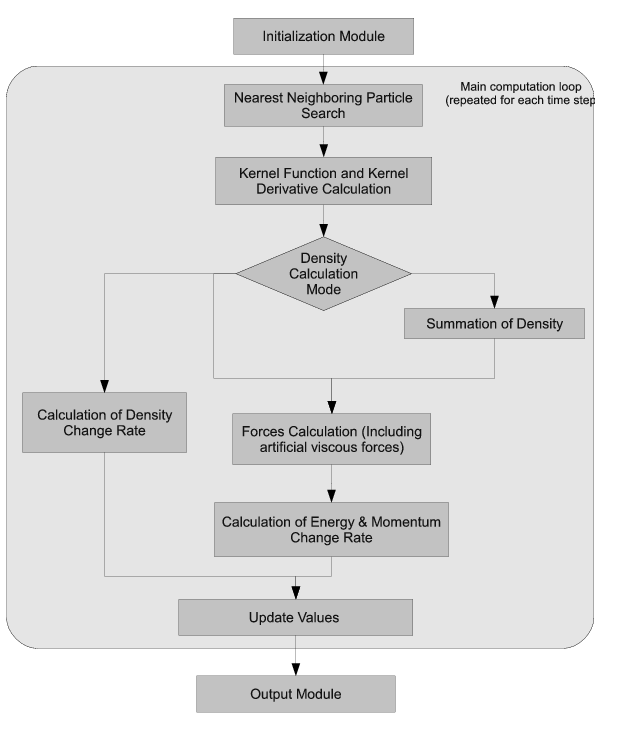
\includegraphics[width=1.0\textwidth]{Graphics/general_structure_SPH}
  \caption{basic structure of an SPH code}
  \label{fig:BasicSphCode}
\end{figure}



\section{Presentation of test cases}
\label{sec:testCases}
 
This section introduces the different test cases, which are used to validate the developped code at the different stages. The general problem setup is presented as well as analytical solutions in case they exist. Otherwise the numerical reference solution is provided.

The reason why this section is placed already here is, that the test problems are sometimes referred to from the code section (\ref{sec:1DSPHcode}, \ref{sec:2DSPHcode}) and it is preferable if they are introduced before.

Details on initializing the flowfield, running the simulations and post--processing are not given in this section but only in section \ref{sec:simuSetupTestCases}, after having introduced the numerical codes. The present section merely povides the basis by introducing equations and the general ideas necessary to perform the actual simulation and the post-processing.

\subsection{1D shock--tube}
As an exact solution is known, the 1D shock tube is a very common test--case for compressible numerical techniques, especially in the form used by Sod \cite{Sod1978}.

%\subsubsection{Presentation and analytical solution}
 The problem consists of two initially separated (e.g. by a diaphragm) gas--filled tube sections, both in general with different properties, at least different pressure. When at the instant $t_0$ (initial situation shown in \ref{fig:shockTubeT0}) the separation is removed, a shockwave is propagating into the low--pressure area and a rarefaction is traveling into the high pressure area, both adjusting the pressure to the same intermediate value. This means that at a time $t_1>t_0$ the situation can be presented as in figure \ref{fig:shockTubeT1} where the nomenclature from Anderson \cite{Anderson2002} is adopted.

\begin{figure}[h]
    \centering
      % Generated with LaTeXDraw 2.0.8
% Tue Aug 31 14:18:55 PDT 2010
% \usepackage[usenames,dvipsnames]{pstricks}
% \usepackage{epsfig}
% \usepackage{pst-grad} % For gradients
% \usepackage{pst-plot} % For axes
\scalebox{1} % Change this value to rescale the drawing.
{
\begin{pspicture}(0,-1.7167188)(12.2,1.7567188)
\psframe[linewidth=0.04,dimen=outer](12.2,0.7032812)(0.0,-1.7167188)
\usefont{T1}{ppl}{m}{n}
\rput(1.775625,-0.51171875){\pscirclebox[linewidth=0.04]{4}}
\usefont{T1}{ppl}{m}{n}
\rput(10.318125,-0.49171874){\pscirclebox[linewidth=0.04]{1}}
\psline[linewidth=0.04cm](6.18,0.68328124)(6.18,-1.6767187)
\psline[linewidth=0.05cm,linestyle=dashed,dash=0.16cm 0.16cm,arrowsize=0.05291667cm 3.0,arrowlength=1.65,arrowinset=0.0]{<-}(6.2,-0.77671874)(7.36,1.0632813)
\usefont{T1}{ppl}{m}{n}
\rput(7.9,1.4082812){\psframebox[linewidth=0.04,framesep=0.1]{diaphragm}}
\usefont{T1}{ppl}{m}{n}
\rput(1.9523437,0.38828126){high pressure section}
\usefont{T1}{ppl}{m}{n}
\rput(10.131719,0.40828124){low pressure section}
\end{pspicture} 
}


      \caption{shock--tube at initial time $t_0$}
      \label{fig:shockTubeT0}

      % Generated with LaTeXDraw 2.0.8
% Tue Aug 31 14:32:35 PDT 2010
% \usepackage[usenames,dvipsnames]{pstricks}
% \usepackage{epsfig}
% \usepackage{pst-grad} % For gradients
% \usepackage{pst-plot} % For axes
\scalebox{1} % Change this value to rescale the drawing.
{
\begin{pspicture}(0,-1.21)(12.2,1.21)
\psframe[linewidth=0.04,dimen=outer](12.2,1.21)(0.0,-1.21)
\usefont{T1}{ppl}{m}{n}
\rput(1.775625,-0.005){\pscirclebox[linewidth=0.04]{4}}
\usefont{T1}{ppl}{m}{n}
\rput(10.318125,0.035){\pscirclebox[linewidth=0.04]{1}}
\psline[linewidth=0.04cm,linestyle=dashed,dash=0.16cm 0.16cm](6.48,1.11)(6.48,-1.15)
\psline[linewidth=0.04cm](8.7,1.17)(8.7,-1.19)
\usefont{T1}{ppl}{m}{n}
\rput(5.3664064,0.015){\pscirclebox[linewidth=0.04]{3}}
\usefont{T1}{ppl}{m}{n}
\rput(7.5034375,-0.005){\pscirclebox[linewidth=0.04]{2}}
\psline[linewidth=0.02cm](4.5,1.19)(4.5,-1.17)
\psline[linewidth=0.02cm](4.56,1.17)(4.56,-1.19)
\psline[linewidth=0.02cm](4.62,1.19)(4.62,-1.17)
\psline[linewidth=0.02cm](4.68,1.17)(4.68,-1.19)
\end{pspicture} 
}


      \caption{shock--tube at time $t_1>t_0$}
      \label{fig:shockTubeT1}
\end{figure}

In figure \ref{fig:shockTubeT1}, areas 2 and 3 are separated by the so called contact discontinuity, which is the fluid interface generated by the removal of the diaphragm. While in general, the states and properties of the fluids in 2 and 3 are different, pressure $p$ and velocity $u$ at both sides of the discontinuity have to be the same:

\begin{equation}
\label{eq:condCD}
p_2=p_3
u_3=u_2
\end{equation}

The analytical solution to the shock--tube problem can be found using the shock relations and the isentropical relations and is taken from Anderson \cite{Anderson2002} as well. 
It will be presented here, as the post processing program, which is described below, is based on this solution.

First the unknown quantities in areas 2 and 3 are calculated (states 1 and 4 are completely known). Then the location of all area boundaries is determined at a certain instant $t_1>t_0$. Finally the properties inside the rarefaction (located between area 3 and 4) can be obtained.

\paragraph{determination of quantities in areas 2 and 3}

With the relation

\begin{equation}
 \frac{p_4}{p_1}=\frac{p_2}{p_1}(1-\frac{(\gamma_4-1)(c_1/c_4)(\frac{p_2}{p_1}-1)}{\sqrt(2\gamma_1*[2 \gamma_1+(\gamma_1+1)(p_2/p_1-1)])})^(\frac{-2 \gamma_4}{\gamma_4-1})
\end{equation}

 the unknown pressure $p_2$ can be determined iteratively, where the sound speed for an ideal gas is calculated according to equation \ref{eq:soundSpeed}. 

For the further proceeding, the ratio of specific heats $\gamma$ is assumed constant (i.e. same gas in 1 and 4 and besides, no variation of $\gamma$ with temperature)

\begin{equation}
 \gamma_4= \gamma_3= \gamma_2= \gamma_1=const
\end{equation}

The density in area 2 can be determined from state 1 with the shock relations 
\begin{equation}
 \rho_2=\rho_1*(1+(\gamma+1)/(\gamma-1)*(p_2/p_1))/((\gamma+1)/(\gamma-1)+p_2/p_1);
\end{equation}

Applying the isentropical relations from state 4, one obtains the density in area 3

\begin{equation}
\rho_3=(p_3/p_4)^(1/gamma)*rho_4
\end{equation}

The internal energy in areas 2 and 3 is obtained by the ideal gas equation of state (\ref{eq:idealGasEqState})

The velocity of the shock traveling into area 1 is
\begin{equation}
\label{eq:shockVelocity}
W=c_1*\sqrt(\frac{(\gamma+1)}{(2*\gamma)}*(\frac{p_2}{p_1}-1)+1)
\end{equation}

With the applicaton of the continuity equation, the velocity induced in area 2 $u_2$ by the shock is
\begin{equation}
 u_2=W*(1-\frac{rho_1}{rho_2})
\end{equation}

Accoring to equation \ref{eq:condCD}, the velocity in area 3 $u_3$ is the same.

\paragraph{determination of the area boundaries at a certain instant}

As geometrical information comes into play, the position of the diaphragm in the space has to be indicated and is assumed to be $x_{dia}=0$ and x is counted positively towards the right (in direction of the low pressure area (area 1)).
The following positions have to be determined (see also figure \ref{fig:shockTubeT1}:

\begin{enumerate} [(a)]

  \item begin rarefaction (delimits area 4) \\
As the begin of the rarefaction propagates into area 4 with the corresponding (local) soundspeed, its position is 
\begin{equation}
 x_{rar,beg}=-c_4 t
\end{equation}

  \item end rarefaction (delimits area 3) \\
The end of the rarefaction propagates with the corresponding (local) soundspeed relative to the fluid in 3 which itself has a velocity $u_3$. The desired position is therefore
\begin{equation}
 x_{rar,end}=(u_3-c_3) t
\end{equation}

  \item contact discontinuity \\
The contact discontinuity moves with the velocity $u_3$ and therefore
\begin{equation}
 x_{CD}=u_3 t
\end{equation}

  \item shock \\
  The expression for the propagation velocity is given by equation \ref{eq:shockVelocity} and therefore
\begin{equation}
 x_{shock}=W t
\end{equation}

\end{enumerate}

\paragraph{determination of the properties inside the rarefaction}
Inside the rarefaction the flow evolves in an isentropic manner, which means the isentropic relation can be employed. Furthermore, the theorie of characteristics gives the velocity at a certain point inside the rarefaction. Again all equations are taken from Anderson ~\cite{Anderson2002} and the coordinate system remains unchanged ($x=0$ corresponds to diaphragm position and therefore origin of rarefaction)

To obtain the velocity inside the rarefactions, the following equation is used
\begin{equation}
 u_{rar}=\frac{2}{(\gamma+1)}(c_4+\frac{x}{t})
\end{equation}

The density at a certain point inside the rarefaction is calculated with
\begin{equation}
\rho=\rho_4 (1-\frac{(gamma-1)}{2}(\frac{u}{a_4}))^\frac{2}{(gamma-1)}
\end{equation}
and for the pressure, the isentropic relation in the following form is used
\begin{equation}
p=p_4(\frac{rho}{rho_4})^\gamma
\end{equation}
Finally, the internal energy is computed with the equation of state \ref{eq:idealGasEqState}.

\subsection{acoustic wave propagation}
Acoustic phenomena play an important role for the actual problem to be investigated within this project (see \ref{sec:intro}). It is therefore necessary to get an idea on how the code reproduces these phenomena. A crucial issue in this context is the damping of oscillating or propagating waves due to numerical dissipation: Many numerical codes have an intrinsic dissipation, intoduced by the numerical scheme, even when the actually implemented equations are inviscid. This numerical dissipation acts like a real viscous dissipation and diminuishes the kinetic energy of the flow. The comparison of the simulation results against the following test cases, whose theoretical solution is always obtained assuming an inviscid flow (i.e. no dissipation), aim at quantifying this damping. A further point to be investigated by means of these test cases is the capability of the code to exactly reproduce the right periodical time $T$ of the propagating/oscillating wave.

In order to quantify the effect of viscosity in the simulation results (no matter what nature it is), a damping factor
is introduced as the relative change in amplitude $A$ of two consecutive periods $i$ and $i+1$
\begin{equation}
 f_d=\frac{A_i-A_{i+1}}{A_i}
\end{equation}
where the amplitude $A$ may be measured either in terms of pressure $p$ or velocity $u$.

For the case of a damping force that is proportional to the velocity, the damping factor
is constant. This fact is important with regard to the artificial viscosity that can be included in the code (see \ref{sec:ArtVisc}). A closer look at the formulation for the artificial viscosity (\ref{eq:MonArtVis}) yields
\begin{equation}
 \Pi_\propto v_{ab}
\end{equation}.
This above statement is made assuming $\nu$ from (\ref{eq:MonArtVis}) constant.



\subsubsection{1D stationnary oscillating wave}
The configuration of an oscillating wave is taken from \cite{Monaghan2005}, where it is used
to study the dispersion relation for an infinite one--dimensional gas. In the present context though, the same configuration is judged suitable for the study of damping and evolution of $T$. 

The sinusoidal oscillation of wavelength $\lambda$ is initialized by a velocity profile with amplitude of 5\% of sound speed
\begin{equation}
 u(x)=0.05 c\sin(2\pi x/\lambda)
\end{equation}
in the domain $0\leq x\leq \lambda$ with periodical boundary conditions on both sides.

For a simple harmonic wave , the theoretical perioiocal time $T$ is given as \cite{Stewart1930}
\begin{equation}
 T=\frac{\lambda}{c}
\end{equation}
and serves as a reference for the comparison with the simulation results.





\subsubsection{1D infinite traveling wave}
This test case is similar to the above one with the difference that now, the wave travels in one direction through the space. A theoretical description for this kind of wave can be found using the wave equation for a velocity potential. This is a linearized equation and therefore valid only for small disturbances, which for the present application is justified.
In Stewart \cite{Stewart1930}, the expressions for the fluctuation (denoted by a $\delta$) of the desired quantities around their mean values (denoted by the subscript $0$) are directly given and read as follows:
\begin{itemize}
\item velocity evolution 
\begin{equation}
\label{eq:1DWaveDetla_u}
 \delta u(x,t)=k A\prime \sin(k(ct-x))
\end{equation}
\item density evolution 
\begin{equation}
 \delta \rho(x,t)=\rho_0\frac{k}{c} A\prime  \sin(k(ct-x))
\end{equation}
\item pressure evolution 
\begin{equation}
 \delta p(x,t)=k c \rho_0 A\prime  \sin(k(ct-x))
\end{equation}
\item evolution of the displacement $\xi=x-x_0$
\begin{equation}
\label{eq:1DWaveDisplacement}
 \xi(x,t)=-\frac{A\prime }{c} \cos(k(ct-x))=-\frac{A\prime }{c} \sin(k(ct-x+\frac{\pi}{2k}))
\end{equation}

\end{itemize}

$A\prime $ denotes the amplitude of the underlying velocity potential and therefore determines the amplitude of the other quantities as well. It can be any random constant with the restriction that the disturubances in $\rho$ and $p$ remain small compared to their mean value (linear theorie). The variable $k$ is the  wavenumber and defined as $k=\frac{2\pi}{\lambda}$.

Furthermore one can note that the displacement is $\pi/2$ or $90°$ in phase ahead of the other quantities. This fact will be important when thinking about the initialization of a finite propagating wave (single wave train). 

For the initialization of the flowfield at the instant $t=0$, the above equations (\ref{eq:1DWaveDetla_u})-(\ref{eq:1DWaveDisplacement}) will be employed (see CORRESPONDING SECTION IN SIMUSETUP...)


\subsubsection{1D wave tain with reflextion and interference}
For the testing of reflextion and interference, the problem as described below is simulated.
But first, some thoughts on the initialization of a single 1D wave train are presented.
Goal is, to initialize a 1D wave train in one part of the domain while the rest shall be initialized with unperturbed flow. For this to make any sense, the size of the domain has of course to be superior to the wavelength $\lambda$ of the wave train. 

First attempts to initialize the single wave train using the equations for a continuous (infinite) traveling wave (\ref{eq:1DWaveDetla_u})-(\ref{eq:1DWaveDisplacement}) have turned out to be problematic due to the phase shift between $\rho,p,u$ on the one hand and the displacement $\xi$ on the other hand. As the wave does not continue indefinitely but is simply cut off after one wavelength, there will always be a discontunuity in one of the quantities.  If, for example, the initialization is done with a smooth transition of $\rho,p,u$ from the unperturbed flow, there is a discontinuity in the displacement, and vice versa. This discontunuity (be it in $\rho,p,u$ or in the displacement) constitutes a new disturbance which again is origin of new waves. So, no neat wave train could be created this way. 
Thus, a different way to generate the wave had to be found and it turned out that the periodic movement of a wall boundary was an appropriate mean to do so. 

Now that single wave trains ca be produced, the test case is introduced:

A domain with size $l_{\mathit{dom}}$ and limited by two solid walls (at $x=0$ and $x=l_{\mathit{dom}}$) is considered. The left hand wall (at $x=0$) has the ability to perform a movement according to a sinusoidal velocity profile, when desired.
The periodical time $T$ of the wave train is chosen in a way that its wavelegth is
$\lambda=l_{\mathit{dom}}/4$. The condition on $T$ is therefore
\begin{equation}
 T=\frac{l_{\mathit{dom}}}{4 c_0}
\end{equation}

The following passage explains the temporal course of the theoretically exact test problem

\begin{itemize} 
\item At $t_0=0$ the left hand side wall begins to move according to 
\begin{equation}
  u_{\mathit{wall}}=u_{\mathit{max}}\sin(\omega t) 
\end{equation}
  where 
\begin{equation}
\omega=2*\Pi/T u_{\mathit{max}}=0.05 c_0
\end{equation}


\item At $t_1=T$ the wall stops moving, meaning that exactly one wave train has been generated, which now travels through the domain

\item At $t_2=l_{\mathit{dom}}/c_0$ the first part of the wave train hits the right hand side  wall and starts being reflected. Simultaniously, the LHS wall starts moving again according to same equation as above, generating a new wave.

\item At $t_3=t_2+T$ the LHS wall stops moving and the generation of the secound wave is finished. 
The first wave is now completely reflected from the RHS wall

\item At $t_4=t_3+T$ the two waves begin to interfere. (Both wave trains reach the middle of the domain)

\item At $t_5=t_4+T/2$ the interference of the waves is at maximum, i.e. both waves interfere along their entire wavelength

\item At $t_6=t_4+T$ the wave interference is over

\item At $t_7=t_6+T$ both waves hit the respective walls. The test problem ends at this instant
\end{itemize}


To get a visual idea of this problem, refer to figure LABEL (show to situations with wave trains...)

 









\section{1D SPH code}
\label{sec:1DSPHcode}

\subsection{Short overview}
PERHAPS THIS SUBSECTION TITLE IS REMOVED AND THE FOLLOWING TEXT WILL FIGURE JUST BELOW THE SECTION TITLE!?!

This code has a relatively simple structure, yet it features all the components
a more sophisticated SPH computational program would incorporate. Both the summation 
density approach and the continuity density approach are implemented (see 
\ref{sec:DensCalcMode}.) By computing a 1D shock tube problem, the code is used to verify 
the basic compressible SPH euler equations which are then implemented in the more complex 2D program. 
As the analytical solution for this problem is well known, the shock tube is a very 
common test case for 1D compressible codes \cite{Sod1978} (PERHAPS ONE MORE REFERENCE WHICH STATES THAT SHOCK TUBE IS A COMMONLY USED TEST CASE...). 
The problem setup and the results obtained are discussed in the corresponding section.

\subsection{Components and structure}
This section introduces all the

\subsubsection{The data structures}

To facilitate the implementation and the handling of the code, two data structures are defined. 

\paragraph{The parameters of the data structure}

This data structure is defined in the header file parameters.h(WRITE IN CODE STYLE) and 
contains all parameters needed to set up the problem. Among those parameters are 
geometrical values, the initial conditions, simulation length and time step 
as well as parameters defining the fluid properties.

\paragraph{The simulation data structure}

Defined in the file simulation.h(WRITE IN CODE STYLE) this structure is made up of all 
variables that change in the course of the simulation. To begin with, these are the 
values of interest like position, velocity, density, pressure, energy, etc.. 
Furthermore there are variables needed as intermediate results (such as the smoothing 
length and its derivative). 
Most of the variables contained in the simulation data structure are needed one per 
particle. Therefore those variables are defined as vectors with a size that corresponds 
to the number of particles in the system. 

\subsubsection{The functions}

As the size of the 1D SPH program is not too big, it admits of the 
introduction/description of every single function used. The textual description is not complete but only comprises particulars and features that are considered worth mentionning. A Nassi-Schneidermann-Diagram (NSD)~\cite{Nassi1973} complements each description and shows the control flow for each function as well as the interdependence of the individual functions. For the sake of a clear illustration, the NSD does not display every loop of the program; frequently, loops over all particles and the interaction list are ommitted (the instruction 'calculate ... for each particle' for example means the implementation of a loop over all particles, i.e., all components of the corresponding variable's vector).  Consulting the comments in the source code is recommended if a more detailed understanding is necessary or desired.

\paragraph{Explanation of a Nassi-Schneidermann-Diagram}
A NSD Diagram is employed in this section as it allows for a more compact description of the code structure within limited space than a conventional flow diagram and, in addition, offers a range of further advantages~\cite{Nassi1973}. It is read from top to bottom, with different box symbols representing different kinds of instructions or control elements. The symbols used during the description of the functions below are the following ones:

\subparagraph{The process symbol}
there has to be some text, otherwise the parcolumns environment will delete the subparagraph heading!?!
\vspace{5mm}
\begin{parcolumns} [colwidths={1=60mm,2=35mm}] {2}  
 
\colchunk{this symbol represents simple instructions for which during their execution no analysis has to be made. Examples are assignments or inputs/outputs. 
A variation of the conventional process box is the symbol for the call of an external function.} 
\colchunk{

\begin{struktogramm}(40,10)
  \assign[10]{\(Instruction\)}
\end{struktogramm}
\vspace{10mm}
\begin{struktogramm}(30,10)
  \sub[10]{\texttt{function()}}
\end{struktogramm}}

\colplacechunks
\end{parcolumns}


% \begin{multicols} [colwidths={1=0.6\textwidth,2=0.35\textwidth}] {2}  
%  
% \colchunk{hhhhhhhhhhhhhhhhhhhhhhhhhhhhhhhhhhhhhhhhhhhhhhhhhhhhhhhhhhhhhhhhhhhhhhhhhhhhhhhhhhhhhhhhhhhhhhhhhhhhhhhhhhhhhhhhhhhhhhhhhhhhhhhhhhhhhhhhhhhhhhhhhhhhhhhhhhhhhhhhhhhhh}
% \colchunk{gggggggggggggggggggggggggggggggggggggggggggggggggggggggggggggggggggggggggggggggggg}
% \colplacechunks
% 
% \end{multicols}

\subparagraph{The iteration symbol}
there has to be some text, otherwise the parcolumns environment will delete the subparagraph heading!?!
\vspace{5mm}
\begin{parcolumns} [colwidths={1=60mm,2=35mm}] {2}  
 
\colchunk{The shown iteration symbol represents loops, where the condition is tested each time before entering the body. This control struct can be implemented by a while loop or a for loop. } 
\colchunk{

\begin{struktogramm}(40,10)
\while[10]{\(while condition true\)}  
\assign[10]{\(body\)}
\whileend
\end{struktogramm}}

\colplacechunks
\end{parcolumns}

\subparagraph{The decission symbols}
there has to be some text, otherwise the parcolumns environment will delete the subparagraph heading!?!
\vspace{5mm}
\begin{parcolumns} [colwidths={1=60mm,2=50mm}] {2}  
 
\colchunk{Control structures that depending on a condition enter different branches, are represented by the decision symbols. A binary decision symbol corresponding to an if-else statement in programming languages is shown in (FIGURE...). For multi branch control structs, such as if-ifelse-...-else or switch-case, (FIGURE...) provides the corresponding symbol (in the example: 3 branches).
 } 
\colchunk{
\sProofOn
\begin{struktogramm}(60,25)
\ifthenelse[10]{6}{6}{condition true?}{Y}{N}
\assign[10]{\(subblock\ 1\)}
\change
\assign[10]{\(subblock\ 2\)}
\ifend
\end{struktogramm}
\sProofOff

\sProofOn
\begin{struktogramm}(60,15)
  \case[15]{3}{3}{\(test\ X\ \ \)}{cond. 1}
        \assign[10]{\(subblock\ 1\)}
    \switch{~2}
        \assign[10]{\(subblock\ 2\)}
    \switch[r]{3~}
      \assign[10]{\(subblock\ 3\)}
   \caseend
\end{struktogramm}
\sProofOff
}
\colplacechunks
\end{parcolumns}
\vspace{5mm}

%this does work in principle, but the figures are not placed exactly at the right position
% \begin{floatingfigure}[v]{50mm}
% \begin{struktogramm}(20,20)[]
% \assign{\(Instruction\)}
% \end{struktogramm}\caption{test}
% \end{floatingfigure}


Remark: The NSD flowchart language provides the possibility to describe programs at their level of implementation. In the following section however, it is used in a more abstract way and instructions or conditions are verbalized. 
 
\paragraph{The Main() function}


As its name suggests, main.cpp(WRITE IN CODE STYLE) is the main function of the program. It is entered upon execution of the program, declares and initializes the data structures and calls the functions needed.

\begin{center}
\sProofOn
\begin{struktogramm}(76,27)[MAIN]
  \assign{\(declare \ parameters\ data\ structure\)}
  \assign{\(declare \leq 4 \ simulation\ data\ structure\)}
  %\sub{\begin{verb} setupSim(param, sims) \end{verb}}
  \sub{\texttt{setupSim(param, sims) }}
  %\sub{\begin{verb} \ marchTime(param, sims)\end{verb}}
  \sub{\texttt{ marchTime(param, sims)}}
  \assign{\(return\ 0  \ (program\ successfully\ ended)\)}
\end{struktogramm}
\sProofOff
\end{center}

\paragraph{The setupSim() function}

Implemented in the file setupSim.cpp (with the corresponding header setupSim.h), this function represents the 'initialization module' from/shown in \ref{fig:BasicSphCode}. More precisely, it first sets up the initial particle distribution for the sepcified problem (which is the Sod shock tube \cite{Sod1978}). Depending on the user's selection made by setting the flag 'constspacing' (member of parameters dara structure), this is done/made? in two different ways:
One possibility is to have an initial particle distribution with the same spacing in the high density area of the shock tube as in the low density area (flag constspacing = true). (REM: THE SHOCK TUBE PROBLEM SHOULD BE INTRODUCED BEFORE (AND NOT AS ORIGINALLY INTENDED ONLY IN THE RESULTS SECTION, AS I HAVE ALREADY REFERRED TO IT SEVERAL TIMES BY NOW...) In this case though, the mass of the particles has then to be adapted to be coherent with the spacing and the initial value of the density.
A second possibility is a particle distribution resulting of a (spatially) constant particle mass (flag constspacing= false). According to the initial value of the density, the particles will then be further apart in the low density area than in the high density area.
For the further course of the program it is essential that each particle has a unique mean of identification. For more sophisticated 2D or 3D codes, this issue is resolved by explicitely assigning each particle an identification number. For this 1D code however, particle identification is already implicitely given due to the way, the particles are represented/stored: The position (consisting only of an $x$ value) of each particle is stored as one component of a position vector X. Therefore the particles can be clearly identified by the number of the vector component they are stored into.

Once the particles are set up, they are assigned their initial values for the shock tube problem as choosen in the parameters.h file.  
\begin{center}
\sProofOn
\begin{struktogramm}(140,115)[SETUPSIM]
  \assign{\(Calculate\ left\ hand\ particle\ spacing\ (dxl)\ based\ on\ constant\ mass\)}
  \assign{\(Calculate\ right\ hand\ particle\ spacing\ (dxr)\ based\ on\ constant\ mass\)}
  \assign{\(Calculate\ particle\ spacing\ (dx)\ for\ constant\ spacing\)}
  \ifthenelse[10]{6}{6}{\(constspacing\ flag==1?\)}{Y}{N}
    \assign[15]{\(place\ particles\ on\ left\ hand\ side\ of \)\linebreak \( problem\ domain\ starting\ at\ center\ (x=0)\ (with\ distance\ dx)\)}
    \assign[15]{\(place\ particles\ on\ right\ hand\ side\ of\)\linebreak \( problem\ domain\ starting\ at\ x=0\ (with\ distance\ dx)\)}
  \change
    \assign[15]{\(place\ particles\ on\ left\ hand\ side\ of\ \)\linebreak \(problem\ domain\ starting\ at\ x=0\ (with\ dinstance\ dxl)\)}
    \assign[15]{\(place\ particles\ on\ right\ hand\ side\ of\ \)\linebreak \(problem\ domain\ starting\ at\ x=0\ (with\ dinstance\ dxr)\)}
  \ifend
  \assign{\(merge\ particle\ positions\ for\ both\ sides\ into\ one\ vector\ x\)}
  \assign{\(create\ vectors\ with\ initial\ values\ for\ u,\ \rho,\ p,\ e,\ m,\ h\ for\ particles\ on\ left\ hand\ side\)}
  \assign{\(create\ vectors\ with\ initial\ values\ for\ u,\ \rho,\ p,\ e,\ m,\ h\ for\ particles\ on\ right\ hand\ side\)}
  \assign{\(merge\ l.h.s.\ and\ r.h.s\ vectors\ into\ one\ single\ vector\ for\ each\ variable\)}
  \ifthenelse[10]{6}{1}{\(constspacing\ flag\ ==\ 1?\)}{Y}{N}
    \assign{\(calculate\ mass\ for\ particles\ on\ left\ hand\ side\)}
    \assign{\(calculate\ mass\ for\ particles\ on\ right\ hand\ side\)}
    \assign{\(merge\ mass\ values\ into\ one\ single\ vector\ \)\linebreak \((overwrite\ mass\ vector\ from\ above)\)}
  \change
  \ifend
  \assign{\(initialize\ vectors\ for\ derivatives\ \ du,\ de,\ d\rho \)}
\end{struktogramm}
\sProofOff
\end{center}




\paragraph{The marchTime() function}

The marchTime function conducts the numerical integration using the leapfrog scheme described in \ref{sec:numIntegr}. If the program runs in the continuity density mode (flag sumdensity = false), the density is integrated as well, whereas if the program runs in the summation density mode (flag sumdensity = true) the density is smoothed. The latter operation is not performed directly in this function but in one of the (sub)functions that it calls.

\begin{center}
 \sProofOn
     \begin{struktogramm}(150,140)[MARCHTIME()]
  \assign{\(initialize\ vectors\ for\ intermediate\ values\ of\  \rho,\ u,\ e\)}
  \while[10]{\(while\ current\ time\ step\ \leq \ number\ of\ total\ time\ steps\)}
    \ifthenelse[10]{6}{1}{\(current\ time\ step\ \neq1\)}{Y}{N}
      \assign{\(save\ current\ values\ for\ \ u,\ e\ in\ their\ intermediate\ variables\)}
      \ifthenelse[10]{6}{1}{\(sumdensity\ flag\ \neq1?\)}{Y}{N}
        \assign{\(save\ current\ rho\ value\)\linebreak \(in\ its\ intermediate\ vector\)}
        \assign{\(calculate\ new\ rho\ (+0.5dt)\ by\ integration\)}
      \change
      \ifend
      \assign{\(calculate\ new\ u,\ e\ (+0.5dt) \)\linebreak \(\ by\ integration\)}
    \change
    \ifend
    \sub{\texttt{calcDerivatives()}}
    \ifthenelse[10]{6}{6}{\(current\ time\ step\ ==1?\)}{Y}{N}
      \ifthenelse{6}{1}{\(sumdensity \neq1?\)}{Y}{N}
        \assign[10]{\(calculate\ new\ \rho\ (+0.5dt)\ by\ inte-\)\linebreak\(gration\)}
      \change
      \ifend
      \assign[10]{\(calculate\ new\ u,\ e\ (+0.5dt)\ by\ integration\)}
      \assign[10]{\(calculate\ new\ position\ x\ (+1.0dt)\)\linebreak\((advance\ particles\ one\ full\ time\ step)\)}
    \change
      \ifthenelse{6}{1}{\(sumdensity \neq1?\)}{Y}{N}
        \assign[10]{\(calculate\ new\ \rho\ (intermediate\ value\  \)\linebreak\(+1.0dt)\ by\ integration\)}
      \change
      \ifend
      \assign[10]{\(calculate\ new\ u,\ e\ (intermediate\ vaules\ \)\linebreak\(+1.0dt)\ by\ integration\)}
      \assign[10]{\(claculate\ new\ position\ x(+1.0dt)\) \linebreak\((advance\ particles\ one\ full\ time\ step)\)}
    \ifend
    \ifthenelse[10]{6}{6}{\(current\ timestep\ \%\ printstep\ ==0?\)}{Y}{N}
      \sub{\texttt{plotShock()}}
    \change
    \ifend
    \assign[10]{\(check\ stability\ criterion\ (max\ velocity\ <\ certain\ limit?)\ and\ if\ necessary:\ exit\ program\)}
  \whileend
     \end{struktogramm}
\sProofOff
\end{center}


\paragraph{The calcDerivatives() function}

This function performs the calculation of the derivatives (or change rates) for the velocity $v$ (equation \ref{eq:VCR_EulerInclArtVis}), the internal energy $e$ (equation\ref{eq:ECR_EulerInclArtVis}) and, if the continuity density appraoch is selected, the density $\rho$(equation\ref{eq:DCR_Euler}). Included in equations \ref{eq:ECR_EulerInclArtVis} and \ref{eq:VCR_EulerInclArtVis} is the artificial viscosity term, which is basically calculated according to equation \ref{eq:MonArtVis}. For the specific case of a shock tube problem however, it is usual to apply artificial viscosity only in zones where particles are approaching each other and to set it to zero in zones where particles are receding. This ensures that the artificial viscosity is used for shocks and not for rarefactions\cite{Monaghan2005}. As the described 1D SPH code is (exclusively) apllied to a shock tube problem, this fact/matter/issue has to be taken into account. 
The criterion for not receding(as there is a $\leq$ in Monaghan05 and not a pure <) particles being 
\begin{equation}
 v_{ab}\cdot r_{ab}\leq 0
\end{equation}
the final expression for the artificial viscosity in this 1D shock tube program is
\begin{equation}
\Pi_{ab}=\begin{cases}
\text{equation \ref{eq:MonArtVis}}, &  \text{for~} v_{ab}\cdot r_{ab}\leq 0 \\
0,&  \text{for~} v_{ab}\cdot r_{ab}> 0 
\end{cases}
\end{equation}

\begin{center}
\sProofOn
\begin{struktogramm}(130,110)[CALCDERIVATIVES()]
  \assign{\(declare\ and\ initialize\ the\ needed\ variables\)}
  \assign{\(reset\ the\ vectors\ d\rho,\ de,\ du\ for\ the\ cnage\ rates\ to\ zero\)}
  \sub{\texttt{calcBuddies()}}
  \ifthenelse[10]{6}{1}{\(sumdensity==1\ or\ first\ time\ step?\ \)}{Y}{N}
    \assign{\(calculate\ \rho\ by\ smoothing:\) \\ \(-\ calculate\ self\ contribution\ for\ each\ particle\ \) \\ \( -\ calculate\ pair\ contribution\)}
  \change
  \ifend
  \assign{\(calculate\ p\ and\ c\ for\ each\ particle\)}
  \while[10]{\(for\ loop\ to\ iterate\ interaction\ list\ for\ calculation\ of\ change\ rates\)}
    \assign{\(calculate\ values\ needed\ for\ artificial\ viscosity\ and\ change\ rates\)}
    \ifthenelse[10]{6}{6}{\(interaction\ pair\ in\ compression?\)}{Y}{N}
      \assign{\(calculate\ artificial\ viscosity\ \Pi_{ab}\)}
    \change
      \assign{\(set\ artificial\ viscosity\ \Pi_{ab}\ to\ zero\)}
    \ifend
    \assign{\(calculate\ contribution\ of\ current\ interaction\ pair\ to\ change\ rates\ du,\ de\)}
    \ifthenelse[10]{6}{1}{\(sumdensity\ \neq1?\)}{Y}{N}
      \assign{\(calculate\ contribution\ of\ interaction\ pair\ to\ change\ rate\ d\rho\)}
    \change
    \ifend
    \assign{\(add\ contributions\ of\ change\ rates\ to\ the\ change\ rate\ variables\ \) \linebreak\((in\ the\ appropriate\ component\ of\ the\ change\ rate\ vectors)\)}
  \whileend
\end{struktogramm}
\sProofOff
\end{center}




\paragraph{The calcBuddies() function}
This function conducts the nearest neighboring particle search as described in \ref{sec:NNPS} using the pairwise interaction method. If two particles $i$ and $j$ constitute an interaction pair, their unique particle ID (see SETUPSIM) is stored in the same component of the vectors pairi and pairj respectively. pairi and pairj belong to the simulation data structure.

\begin{center}
\sProofOn 
\begin{struktogramm}(130,90)[CALCBUDDIES()]
  \assign{\(initialize\ the\ varibales\ to\ zero\ \)\\\((components\ of\ the\ two\ vectors\ pairi,\ pairj\ constituing\ the\ interaction\ list,\)\\ \(\ the\ counter\ for\ the\ total\ number\ if\ interactions,\ \) \\ \(the\ vectors\ containing\ w\ dW\ for\ each\ interaction\ pair,\)\\ \(...)\)}
  \while[10]{\(loop\ from\ first\ to\ penultimate\ particle\)}
    \while[10]{\(loop\ from\ second\ to\ last\ particle\)}
      \ifthenelse[10]{6}{1}{\(are\ particles\ interacting?\)}{Y}{N}
        \assign{\(increment\ counter\ of\ total\ interactions\ niac\)}
        \assign{\(save\ the\ particle's\ IDs\ in\ the\ vectors\ pairi\ and\ pairj\)}
        \assign{\(calculate\ kernel\ value\ W_{ab}\ and\ derivative\ dW_{ab}\)\\\( for\ interaction\ pair\)}
        \ifthenelse[10]{6}{1}{\(niac\ \geq max.\ admissible?\)}{Y}{N}
          \assign{\(output\ message\ on\ screen\ and\ exit\ program\)}
        \change
        \ifend
      \change
      \ifend
    \whileend
  \whileend
\end{struktogramm}
\sProofOff
\end{center}


\paragraph{The W() function}
The W() function implements the smoothing kernel for the SPH method, which in this case is the cubic spline kernel (see \ref{sec:KernelFunction}). For implementation purposes the expression of this kernel function (\ref{eq:cubicSpline}) has been expanded resulting in

\begin{equation}
\label{eq:cubicSplineImplement}
M_{4}(x)=\begin{cases}
\frac{2}{3}-q^{2}+0,5q^{3},& \text{for 0 $\leq$ q $\leq$ 1} \\
\frac{1}{6}(2-q)^{3},&  \text{for 1 $\leq$ q $\leq$ 2} \\
O,& \text{for q $>$ 2}
\end{cases}
\end{equation}

\begin{center}
\sProofOn
\begin{struktogramm}(100,31)[W()]
  \case[15]{3}{3}{\(test\ distance\)}{\(is\ distance\ >2?\)}
        \assign[10]{\(W\ according\ to \ \)\\(eq:\ref{eq:cubicSplineImplement})}
    \switch{\(<1?\)}
        \assign[10]{\(W\ according\ to \ \)\\(eq:\ref{eq:cubicSplineImplement})}
    \switch[r]{\(else\)}
      \assign[10]{\(W\ according\ to \ \)\\(eq:\ref{eq:cubicSplineImplement})}
    \caseend
  \assign{\(return\ W\)}
\end{struktogramm}
\sProofOff
\end{center}

\paragraph{The dW() function}
The derivative of the smoothing kernel $\frac{dW}{dx}$ (in 1D) is calculated by this function. Based on the definition of the cubic Spline Kernel(\ref{eq:cubicSpline}), this derivative can be determined easily as

\begin{equation}
\label{eq:cubicSplineDer}
M_{4}(x)=\begin{cases}
\-2q+1,5q^2,& \text{for 0 $\leq$ q $\leq$ 1} \\
-\frac{1}{2}(2-q)^{2},&  \text{for 1 $\leq$ q $\leq$ 2} \\
O,& \text{for q $>$ 2}
\end{cases}
\end{equation}

\begin{center}
\begin{struktogramm}(100,31)[dW()]
  \case[15]{3}{3}{\(test\ distance\)}{\(is\ distance\ >2?\)}
        \assign{\(dW\ according\ to \ \)\\(eq:\ref{eq:cubicSplineImplement})}
    \switch{\(<1?\)}
        \assign{\(dW\ according\ to \ \)\\(eq:\ref{eq:cubicSplineImplement})}
    \switch[r]{\(else\)}
      \assign{\(dW\ according\ to \ \)\\(eq:\ref{eq:cubicSplineImplement})}
    \caseend
  \assign{\(return\ dW\)}

\end{struktogramm}
\end{center}

\paragraph{The plotShock() function}
This function corresponds to the output module as shown in \ref{fig:BasicSphCode} and writes the simulation results at a certain time step in a file named 'dataStepxxxxxx.txt, where xxxxx means the corresponding time step. The frequency of the output can be choosen by editing the parameter printstep (IN CODE STYLE) of the parameter data structure. Each output file has the following format:

$x$ $\rho$ $p$ $u$ $e$
(one line for each particle)
(INSERT A TABLE FOR THE FILE STRUCTURE OR DIRECTLY A CAPTION OF THE TXT FILE...)
\vspace{5mm}
\sProofOn
\begin{struktogramm}(127,60)[PLOTSHOCK()]
  \assign{\(create\ name\ for\ the\ output\ file\ ('dataStepxxxxxx.dat')\)}
  \assign{\(create\ outputfile\ itself\)}
  \while[10]{\(loop\ over\ all\ particles\ (i=0\ until\ i<np)\)}
    \assign{\(output\ component\ i\ of\ the\ position\ vector\ in\ file\)}
    \assign{\(output\ component\ i\ of\ the\ density\ vector\ in\ file\)}
    \assign{\(output\ component\ i\ of\ the\ pressure\ vector\ in\ file\)}
    \assign{\(output\ component\ i\ of\ the\ velocity\ vector\ in\ file\)}
    \assign{\(output\ component\ i\ of\ the\ internal\ energy\ vector\ in\ file\)}
    \assign{\(linebreak\ in\ file\)}
    \assign{\(increment\ i\ (next\ particle\)}
  \whileend
\end{struktogramm}
\sProofOff


\section{2D SPH code}
\label{sec:2DSPHcode}
\subsection{short overview}
The 2D SPH code is more sophisticated than the formerly introduced 1D code. Features such as different types of boundary conditions, a more complex and more efficient neighbouring particle search allgorithm , physical viscosity description and heat conduction, as well as an automatic time stepping control are implemented. Thus, this program is more flexible and can be used to treat problems of real scientific and practical importance. 

Just like the 1D SPH code, the 2D code is implemented in C++. While the 1D code is still using a functional programming approach, the 2D code follows the object-oriented programming paradigm.

But before starting to describe the structure of the code including all the objects and their interaction (subject of the following paragraphs), a short introduction on the file structure of the whole repository, which containins code, pre-- and post--processing scripts, results etc. is given.

The main folder is called {\tt sph-blitz} and contains a number of sub--folders. Those folders, that are important for the use of the program, are briefly detailed here. The others contain different add--ins and third--party libraries for the program, but their detailed knowledge is not required.
While Information on how to install and run the program is given in the corresponding section (\ref{sec:HowToInstAndRun2D}), the present description shall be considered as a first orientation guide. It should help the user to get a rough idea on where to find what.
\begin{itemize}
 \item {\tt src}\\
This folder contains the source code of the c++ program. It has again several subfolders, some of which with further source-files that have been grouped together.
Furthermore it contains a folder {\tt html} f
Finally there is also a folder {\tt outdata}, where the simulation results are written to. This folder might not exist by default. In this case it is automatically created during simulation. 
\item {\tt scripts}\\
Scripts necessary for pre--processing (generation of initial particle distributions) as well as for post--processing  are arranged in this folder
\item{\tt gnuplot}\\
Gnuplot being the name of a plotting--software, this folder contains gnuplot--scripts for visualization of the results.

\end{itemize}
Some of the folders and subfolders contain README--files, which can be consulted for more precise information and instructions on the corresponding subject. But before having a look at these, it is recommended to read over section \ref{sec:HowToInstAndRun2D}), as many issues are adressed there.









\subsection{components}
Describe doxygen

\subsection{structure}

\lstinputlisting[language=c++,caption=An example of program listing,captionpos=b]{code/hello.cpp}

\subsection{How to install and run the program}
\label{sec:HowToInstAndRun2D}


\section{simulation Setup for different test cases}
\label{sec:simuSetupTestCases}



\chapter{Results}
\section{1D SPH code}
...Monaghan05 p.1739... not shock width important but pre and after shock values...

\section{...}
\label{sec:results}

In the Figure~\ref{fig:1dshock} one can see \ldots

\begin{figure}[h]
  \centering
  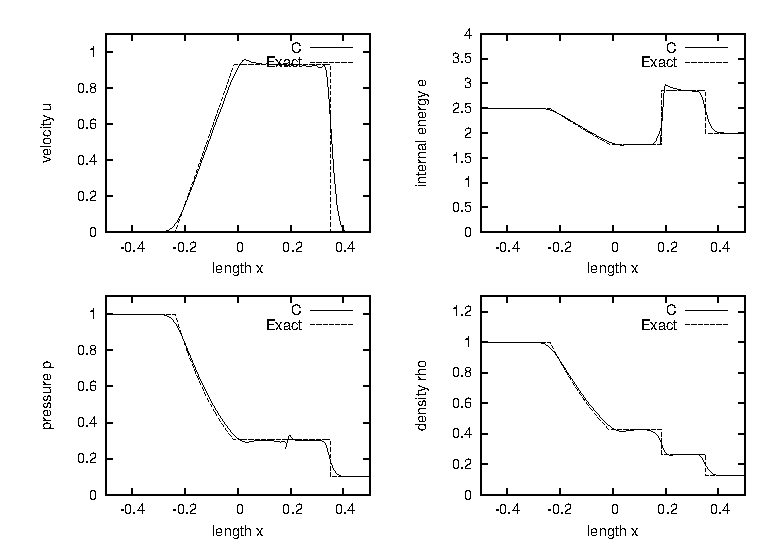
\includegraphics[width=0.95\textwidth]{img/1dshock.eps}
  \caption{An example of a figure}
  \label{fig:1dshock}
\end{figure}

\section{2D SPH code}



\chapter{Conclusion}
\label{sec:conclusion}

\listoffigures

\bibliography{bibdata}
\bibliographystyle{plain}

\end{document}

